%! Author = Len Washington III
%! Date = 9/12/2023

% Preamble
\documentclass[22]{cs430lecture}

% Packages

% Document
\begin{document}

%<*Lecture-Activity-22>
\maketitle
\section{Fibonacci Heaps}\label{sec:fibonacci-heaps}
Fibonacci heaps which support heap operations that do not delete elements in constant amortized time.
From a theoretical standpoint, Fibonacci heaps are especially desirable when the number of \Call{Extract-Min}{} and \Call{Delete}{} operations is small relative to the number of other operations performed.
This situation arises in many graph algorithms.\\

In essence, a Fibonacci heap is a ``lazy'' binomial heap in which the necessary housekeeping is delayed until the last possible moment: deletion.
\begin{table}
    \centering
    \begin{threeparttable}
		\label{tab:}
		\begin{tabular}{|l|l|}
			\toprule
			\begin{minipage}{0.5\textwidth}
				\begin{itemize}
					\item Set of Heap ordered trees (each parent smaller than children).
					\item Maintain pointer to minimum element (\Call{Find-Min}{} takes $O(1)$ time).
					\item Set of marked nodes (if one of its children has been removed).
					\item $n$ - number of nodes in the heap.
					\item \Call{Rank}{$x$} -- number of children of node $x$.
					\item \Call{Rank}{$H$} -- Max rank of any node in heap $H$.
					\item \Call{Trees}{$H$} -- Number of trees in heap $H$.
					\item \Call{Marks}{$H$} -- number of marked nodes in $H$.
				\end{itemize}
			\end{minipage} & \begin{minipage}{0.5\textwidth}
				\begin{figure}[H]
											 \centering
											 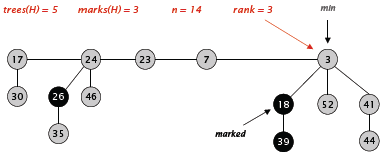
\includegraphics[width=\textwidth]{22.1}
											 \label{fig:22.1}
				\end{figure}
			\end{minipage}\\
			\bottomrule
		\end{tabular}
	\end{threeparttable}
\end{table}

\begin{enumerate}
    \item See \url{https://www.cs.usfca.edu/~galles/JavascriptVisual/FibonacciHeap.html} and \url{https://www.cs.princeton.edu/~wayne/cs423/fibonacci/FibonacciHeapAnimation.html} to help describe how each operation is done, and a rough estimate on its run time:
\end{enumerate}

\binomialqueueop{Make-Heap}
\oldanswer{$O(1)$ Makes a single node heap.}

\binomialqueueop{Insert}
\oldanswer{$O(1)$ Make single node heap, put in the (bidirectional linked) list to left of current min.
Update min pointer if necessary.}

\binomialqueueop{Minimum}
\oldanswer{$O(1)$ We maintain a pointer to the min.}

\binomialqueueop{Union}
\oldanswer{$O(1)$ Link the two root lists together%
\footnote{You don't need to walk either to do that.}%
, and then update the min pointer to point to the smaller of the two previous mins.}

\binomialqueueop{Extract-Min}
\oldanswer{Find min is $O(\log n)$%
\footnote{The name Fibnoacci comes from the fact that the base in the $\log n$ is the golden ratio. The maximum degree of any node in the root list is also related to Fibonacci.}
because we have a pointer to the min.
Remove min from root list (saving the value to return).
If the min had children, put those children in the root list.
\Call{Consolidate}{} the root list%
\footnote{Use array of rank on last node}}

\binomialqueueop{Decrease-Key}
%\oldanswer{``Walk it up''.
%The maximum height is $O(\lg n)$.
%If get up to root list, check if new node in root list is smaller than the current min, if so, move the min pointer.}
\oldanswer{$O(1)$ Reduce value at that node, move it and its subtree to root list, check if new min value pointer.
Breaking that binomial heap by removing a subtree%
\footnote{Do not \Call{Consolidate}{} yet.}.
Wait for a marked node to lose a 2nd child, move to root list, don't \Call{Consolidate}{} yet.
}

\binomialqueueop{Delete}

\begin{table}%
    \centering%
    \begin{threeparttable}%
		\label{tab:}%
		\begin{tabular}{|l|l|}%
			\toprule%
			\begin{minipage}{0.71\textwidth}%
				\begin{table}[H]%
				    \centering%
					\label{tab:operations}%
					\begin{tabular}{|l|c|c|c|}%
						\toprule%
						Operation & Binary Heap & Binomial Heap & Fibonacci Heap\\
						\midrule
						\Call{Make-Heap}{}		& $\theta(1)$		& $\theta(1)$ 		&  $\theta(1)$ \\
						\Call{Insert}{}			& $\theta(\log n)$	& $\theta(\log n)$ &  $\theta(1)$ \\
						\Call{Minimum}{}		& $\theta(1)$		& $\theta(\log n)$ &  $\theta(1)$ \\
						\Call{Extract-Min}{}	& $\theta(\log n)$	& $\theta(\log n)$ &  $\theta(\log n)$ \\
						\Call{Union}{}			& $\theta(n)$		& $\theta(\log n)$ &  $\theta(1)$ \\
						\Call{Decrease-Key}{}	& $\theta(\log n)$	& $\theta(\log n)$ &  $\theta(1)$ \\
						\Call{Delete}{}			& $\theta(\log n)$	& $\theta(\log n)$ &  $\theta(\log n)$ \\
						\bottomrule
					\end{tabular}
				\end{table}
			\end{minipage} & \begin{minipage}{0.29\textwidth}
				Note that the times indicated for the Fibonacci heap are amortized times while the times for binary and binomial heaps are worst-case per-operation times.
			\end{minipage}\\
			\midrule
		\end{tabular}
	\end{threeparttable}
\end{table}


%</Lecture-Activity-22>

\end{document}